\documentclass[a4paper]{article}
\usepackage[top=1in, bottom=1.25in, left=1.25in, right=1.25in]{geometry}
\usepackage{amsmath}
\usepackage{multicol}
\usepackage{graphicx}
\usepackage[utf8]{inputenc}
\usepackage[english]{babel}
\setlength{\parskip}{0.03cm plus4mm minus3mm}
\RequirePackage{ltxcmds}[2010/12/07]
%opening
\title{MQAM system}

\begin{document}
	\maketitle
	
The MQAM system has four components: a transmitter designated MQAM transmitter, a communication channel and two sinks. 

The MQAM transmiter generates two output signals: an optical and a binary signal. The optical signal is transmitted through the communication channel to one of the sinks that works as a receptor and is designated MQAM receptor. The binary signal is used in the other sink to measure the Bit Error Rate (BER). This transmitter doesn't accept any input signal.
	
\section*{MQAM transmitter}

The MQAM transmitter has seven blocks:

\begin{itemize}
	\item Binary Source (B1)
	\item MQAM Mapper (B2)
	\item Discrete to Continuous (B3, B4)
	\item Pulse Shaper (B5, B6)
	\item IQ Modulator (B7)
\end{itemize}

\begin{figure}
	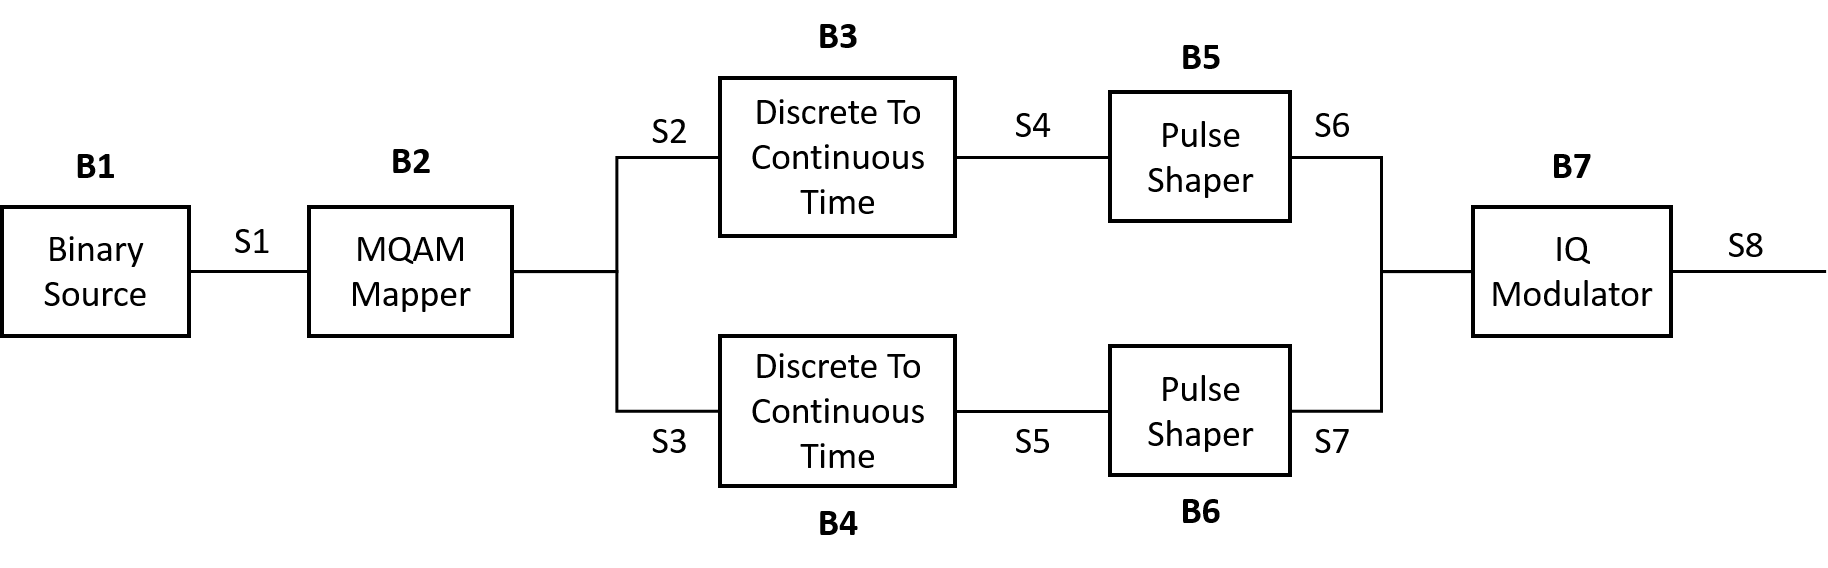
\includegraphics[width=1.2\textwidth]{MQAM_transmitter_block_diagram}
	\caption{MQAM transmitter block diagram}
	\label{MQAM_system_block_diagram}
\end{figure}

Each of the Bi (i=1,...,7) blocks represents a block of code that executes a specific task. A detailed description of these blocks can be found in the \textit{lib} repository. Figure \ref{MQAM_system_block_diagram} represents the transmitter in a schematic manner.

\subsection*{Functional description}

The MQAM transmitter produces two output signals: an optical and a binary signal. 

The optical signal can be scalar or have two polarization components along two perpendicular axis. To generate the optical signal it starts with a binary signal generated by the \textit{binary source}. This signal is then mapped in the IQ space by the \textit{MQAM mapper} block producing two signals: one in phase and one in quadrature. Each one of these signals is converted into a continuous signal in the time domain by the \textit{DiscreteToContinuous} blocks and then filterd in the \textit{Pulse Shaper} block. Lastly the \textit{IQ modulator} blocks recombines the two signals in order to produce a complex optical signal.

The binary signal is extracted directly froom the \textit{binary source} block.

\section*{Communication channel}

The communication channel has only thermal noise.

\section*{MQAM receptor}

\section*{BER measurement}

\end{document}